\documentclass{llncs}
%%%%%%%%%%%%%%%%%%%%%%
%%%%   PACKAGES   %%%%
%%%%%%%%%%%%%%%%%%%%%%
\usepackage{makeidx}
\usepackage{amsmath}
\usepackage{amssymb}
\usepackage{stmaryrd}
\usepackage{graphicx}
\usepackage{subfigure}
\usepackage{latexsym}
\usepackage{url}
\usepackage{color}
\usepackage{isabelle}
\usepackage{isabellesym}
\usepackage{theorem}
\usepackage{multicol}
\usepackage{algorithmic}
\usepackage[linesnumbered,ruled,vlined]{algorithm2e}
\usepackage{multicol}
%%%%%%%%%%%%%%%%%%%%%%%%%%%%
%For Isabelle code
\newlength{\fminilength}
\newsavebox{\fminibox}
\newenvironment{fmini}[1][\linewidth]
  {\setlength{\fminilength}{#1\fboxsep-2\fboxrule}%
   \vspace{2ex}\noindent\begin{lrbox}{\fminibox}\begin{minipage}{\fminilength}%
   \mbox{ }\hfill\vspace{-2.5ex}}%
  {\end{minipage}\end{lrbox}\vspace{1ex}\hspace{0ex}%
   \framebox{\usebox{\fminibox}}}

\newenvironment{specification}
{\noindent\scriptsize
\tt\begin{fmini}\begin{tabbing}X\=X12345\=XXXX\=XXXX\=XXXX\=XXXX\=XXXX
\=\+\kill} {\end{tabbing}\normalfont\end{fmini}}
\def \twoSpaces {\ \ }
%%%%%%%%%%%%%%%%%%%%%%%%%%%%

%%%%%%%%%%%%%%%%%%%%%%%%%%%%
%for comments
\newcommand\JP[1]{\textcolor{magenta}{JP: #1}}
\newcommand\lyj[1]{\textcolor{green}{lyj: #1}}
\def \pInv {i}

\def \twoSpaces {\ \ }
\def \oneSpace {\ }
\def \eqc {\doteq }
\def \andc {\barwedge }
\def \negc {!}
\def \orc {\veebar }
\def \alt {$/\backslash$ }
\def \cat {\symbol{94}}

\def \dbRight {$\backslash\backslash$}
\def \iInv {iInv}
\def \iR {iR}
%%%%%%%%%%%%%%%%%%%%%%%%%%%%
%\def \pInv1 {i2}
%\def $\wedge$ {$\wedge$}
%\def $\Rightarrow$ {$\Rightarrow$}
%\def  \<equiv> {$\equiv$}
%%%%%%%%%%%%%%%%%%%%%%%%%%%

%%%%%%%%%%%%%%%%%%%%%%%%%%%
% Additional math operators
%%%%%%%%%%%%%%%%%%%%%%%%%%%

\usepackage[colorlinks,
            linkcolor=black,
            anchorcolor=black,
            citecolor=blue,
            urlcolor=black,
            bookmarks=true
            ]{hyperref}

%\input{tcilatex}

%=========================================
\begin{document}

\title{  An Automatical Parameterized Verification of  FLASH Cache Coherence Protocols by Paraverifier}
\titlerunning{paraVerifier: An Invariant Finder}
\author{~}
\authorrunning{~}
\institute{~}

\maketitle

%-------------------------------------------------------------------------
\begin{abstract}
%-------------------------------------------------------------------------
The FALSH protocol is an industrial-scale cache coherence protocol, whose parameterized verification is a notoriously hard challenge to the field of formal methods. In this paper, we show how to verify its important properties by our tool {\sf paraverifier}. Being distinguished from any other approach, our proof product are a formal  proof with a set of inductive invariants. %by induction in Isabelle and a series of message flows which reflect the semantics of the protocol intuitively.
Among all the work, our work is the most automatical, and the the set of auxiliary invariants is the most complete. Both invariants are searched automatically and the formal proof is generated automatically. Besides, we make efforts to illustrate the semantical intuition behinds these invariants.
%delay and early versions of FLASH protocol are verified, and the differences between the two versions can be reflected in the auxiliary invariants and flow charts for them found by the tool.

%-------------------------------------------------------------------------
\end{abstract}
%-------------------------------------------------------------------------

%=========================================
\section{Introduction}
%=========================================
Verification of parameterized concurrent systems is interesting in
the area of formal methods, mainly due to the practical importance
of such systems. Parameterized systems exist in many important
application areas: cache coherence protocols, security systems, and
network communication protocols, \emph{etc}. In this work, we will
focus on a cache coherence protocol -FLASH. The challenge posed by
parameterized verification is that the desired properties should
hold in any instance of the parameterized system. %The core of
%parameterized verification is the construction of a set of auxiliary
%invariants~\cite{Pnueli2001,Chou2004,Pandav2005,cubicle2011}, which
%are either used for inductive verification or abstraction model
%construction. Therefore, how to find these auxiliary invariants is
%the central problem in the research field of parameterized
%verification.
%\JP{It is unclear what is the initial invariant and what are the correctness proofs.}
%\JP{To make the concepts clear, it will be better to briefly describe the standard
%procedure for parameterized verification.
%Then you can talk about initial invariant, correctness proofs, auxiliary invariants, etc.
%(Such terms are not explained so far in the current paper.)}
%\JP{Here, still the statement of the research problem is missing.
%Why an invariant finder is needed (the motivation)?}

Stanford FLASH cache coherence protocol \cite{FLASHCache} is a publicly-recognized challenging benchmark in the field of formal
 verification. In the pioneering work,
Park and Dill applied the general purpose theorem prover PVS\cite{cade92-pvs}
to   verifing the protocol for arbitrary $N$ nodes\cite{Park1996a}. This is a laborious process, since they introduce a simplified  FLASH protocol with the so-called aggregated transactions, which
is in fact an abstracted version of FLASH, and  need prove
the correspondence between the abstract and the original FLASH
protocol, and then prove the correctness of the abstracted protocol, and subsequently derive the correctness of  the
original protocol by the correspondence. New   auxiliary state variables
like {\tt fwdSrc} are   introduced  for verification. Deep human insight for FLASH is needed for both the construction of the abstracted protocol  and  introducing new state variables. Inductive invariants must also be
 provided by human, and the theorem prover must be manually guided to perform the induction proof to prove the correspondence between the aggregated protocol  and the original one. %This work is really pioneering because later research on FLASH must also rely on the version of FLASH in \cite{}. Especially, the auxiliary
%variables proposed  are reserved and needed for verification in later work.

Mcmillan applies methods of compositional model
checking \cite{McMillan2001} to the verification of FLASH by using Candence-SMV \cite{cadenceSMV}. %This approach has the advantage that parameterized
%systems can be proved correct without the need to state inductive invariants explicitly,
%since invariant information is obtained by model checking abstract systems.
Safety and liveness of the
FLASH protocol are both verified. Despite the fact SMV is designed as a model-checker to automatically checking properties, the core techniques for FLASH parameterized verification adopted by Mcmillan is SMV's advanced features for proof such as composition proof and temporal case splitting, and abstraction. Human interaction must be heavily relied on to  guide SMV to work, depending on his deep insight to FLASH. Unlike a general theorem prover like Isabelle, SMV does not have a good logical foundation and mechanism to perform theorem proving. The above proofs are neither rigorous as a theorem prover, nor easily understood to a non-specialist of SMV.  Because these proof techniques is only special for SMV,  they are  difficult to be generalized to other protocols and to be implemented in a general-purpose theorem prover.

The CMP method, which adopts parameter abstraction and guard strengthening, is proposed
in~\cite{Chou2004} for verifying a safety property $inv$ of
a parameterized system.
 An abstract instance of the parameterized protocol,  which consists of m + 1
nodes $\{P_1, \ldots , P_m, P^*\}$ with $m$ normal nodes plus one
abstract node $P^*$, is constructed iteratively. The abstract system is an
abstraction for any protocol instance whose size is greater than
$m$. Normally the initial abstract system does not satisfy the
invariant $inv$. Nevertheless it is still submitted to a model
checker for verification. When a counterexample is produced, people need to
carefully analyze it and come up with an auxiliary invariant
$inv'$, then use it to strengthen the guards of some transition
rules of the abstract node. The `strengthened' system is then
subject to model checking again. This process stops until the
refined abstract system  eventually satisfies the original invariant
  as well as all the auxiliary invariants supplied by people. However, this method's soundness is only argued in an
informal way. To the best of our knowledge, no one has
formally proved its correctness in a theorem prover. This
situation may be not ideal because its application domain for cache
coherence protocols  which demands the highest assurance for
correctness. Besides, the analysis of counter-example and generation of new auxiliary invariants usually
 depend on human's deep insightful understanding of the protocol. It is too laborious for people to do these analysis and some effective automatic  tool is needed to help people.

In \cite{cubeicBeyond}, an algorithm, called BRAB,    computes over-approximations of
backward reachable states that are checked to be unreachable in
a finite instance of the system. These approximations (candidate
invariants) are then model checked in together with the original
safety properties. A Finite instance (even small) is regarded as
an oracle for guiding the choice of candidate
invariants. Auxiliary invariants are found automatically, but these auxiliary invariants are in concrete form, and are not generalized to the parameterized form. Thus there is no  parameterized proof derived for parameterized verification. Until now, we still can not find a completely formal proof is constructed to verify the full-version of FLAH protocol by adopting the invariants computed by BRAB. %Our work differs from this work in two main points: (1) we  propose three kinds of causal relations and consistency lemmas, which guide the tool to find invariants and construct an inductive proof; (2) we also develop a system approach to generalize the found concrete invariants and causal relations into a symbolic proofs for parameterized verification. For the full version of FLASH protocol with data path, the   invariants computed by BARB are different from ours. Until now, we still can not find a completely formal proof is constructed to verify the full-version of FLAH protocol by adopting the invariants computed by BRAB.

To sum up,  FLASH is a hard  benchmark with significance for any proposed method for parameterized verification. First it is a cache coherence protocol in real-world, which is  the most important landmark in this field.  As Chou, Mannava, Park pointed out in their FMCAD 2004 paper \cite{Chou2004}, ��if the method works on FLASH, then there is a good chance that it will also work on many real-world cache coherence protocols��. Second
FLASH protocol is  sufficiently hard that only two or three methods have  fully verify
the protocol parametrically. However, human guidance still plays a key role in these successful verification for FLASH. This fact reveals  the weakness of automatical tool in the parameterized verification.  Third, further  efforts are still needed for clear mechanization. As argued in \cite{Chou2004}, ``the first priority is clearly mechanization. Ideally, we want to formalize not only the reasoning
steps  but also the theory developed in a theorem
prover, so that we can have a completely formal proof". Therefore it is preferable to  have a completely formal proof for verification of FLASH in a well-known theorem prover. Previous work is too far away from giving a formal proof for FLASH. Even for a moderate case GERMAN protocol, which is much simpler than FLASH, no formal proof is not available yet. Let alone FLASH.


The aim of this paper is to apply {\sf paraVerifier} to a  parameterized verification of FLASH protocol in both an automatical and rigorous way. In detail, 
\begin{itemize}
\item Interesting auxiliary invariants can be found by {\sf paraVerifier} automatically. Our invariants are visible, which can characterize the semantical features of FLASH, and help people to precisely understand the design of   FLASH.

\item With the help of {\sf paraVerifier}, a formal proof can be constructed automatically as a product of a parameterized verification of FLASH. The formal proof script not  only models the protocol rigorously and specifies its properties without any ambiguity, but also proves them mechanically in the theorem prover. Therefore, it helps us to achieve the highest possible assurance for the correctness of FLASH.
    
   
\end{itemize}

The organization of this work is as follows: Section \ref{sec:Preliminaries} introduces the background of {\sf paraVerifier}; Section  \ref{sec:informalOfFLASH} introduces informally FLASH protocol; Section \ref{sec:formalDescription} introduces our FLASH model in Murphi\cite{Dill1996}; Section \ref{sec:experiments} shows our verification experiments in detail. Especially we introduce some advanced techniques used in our experiments: oracles of simplified version and hybrid oracles, and distributing oracles. Section \ref{sec:relatingWithFlow} tries to explain meanings of inductive invariants with flows.  Section \ref{sec:conclusion} concludes our work.

%=========================================
\section{The Background  of {\sf paraVerifier}\label{sec:Preliminaries}}
%=========================================
{\sf paraVerifier} is devoted to the parameterized verification of a protocol. Usually the tool is used to prove the correctness of the protocol after model checking or testing techniques have been used to verify that typical protocol instances of the protocol  is bug-free. There is still a big gap between the bug-freeness in quite a small number of instances between the correctness in all instances.  Ideally, a proof is preferable to be given to  prove that the correctness holds for any instance. It is a formal proof in a theorem prover that {\sf paraVerifier} generates to verify the protocol. In order to achieve this aim, {\sf paraVerifier} is designed with the following features.

\paragraph{Theoretical foundation}  {\sf paraVerifier} is based on a simple but elegant theory.  Three kinds of causal
relations among a rule and an invariant and a set of invariants are introduced, which are
essentially special cases of the general induction rule. Then, a
so-called consistency lemma is proposed, which is the cornerstone in
our method. Especially, the theory foundation itself is  verified as a
formal theory in Isabelle, which is the formal library for verifying protocol case studies. The library provides basic types and constant definitions to model protocol cases and lemmas to prove  properties.  Therefore, the theoretical foundation itself is verified in Isabelle. Thus it is the most rigorous.

Tool {\sf paraVerifier} is composed of two parts:  an invariant finder {\tt invFinder}
and a proof generator {\tt proofGen}. An overview of our method is  illustrated in Fig.~\ref{fig:arch}.


\begin{figure}[htbp]
\centering %
%\vspace{-0.8cm}
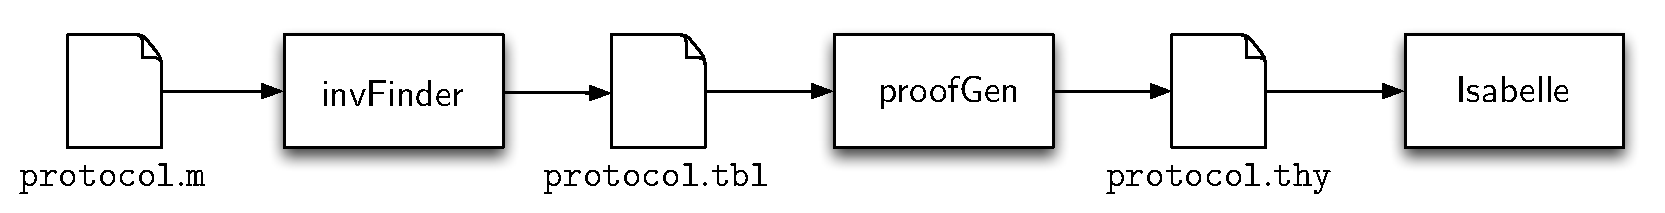
\includegraphics[width=1\textwidth]{paraVerifier.pdf}
\vspace{-0.6cm}
\caption{The workflow of {\sf paraVerifier} \label{fig:arch}
}
\end{figure}

\paragraph{invFinder}%In order to verify  that an
%invariant $inv$ holds for any parameterizd instance of a protocol.
Given a protocol $\mathcal{P}$ and a property $inv$,  written in
a Murphi  file {\tt prot.m}, is compiled into an internal form {\sf prot.ml}, then fed into the
\texttt{invFinder}. {\tt invFinder} automatically transform the Murphi file into internal formal model in Ocaml, then tries to find useful auxiliary invariants and causal relations which are capable of proving $inv$. To construct auxiliary invariants and causal relations, we employ heuristics inspired by consistency relation. Also, when several candidate invariants are obtained using the heuristics, we use oracles such as NuSMV and Murphi model checker and an SMT-solver to check each of them under a small reference model of $\mathcal{P}$, and chooses the one that has been verified in the oracles. A table {\tt prot.tbl} is worked out  to store the set of ground invariants and
 causal relations.


\paragraph{proofGen} For the auxiliary invariants and causal relations stored in table {\tt prot.tbl}, {\tt proofGen} generalizes them  into a parameterized form, which are then used to construct a completely parameterized formal proof in a theorem prover (e.g., Isabelle) to model $\mathcal{P}$ and to prove the property $inv$. After the base theory is imported, the generated proof is checked automatically.  Usually, a proof is done interactively. Special efforts in the design of the proof generation are made in order to make the proof checking automatically.





\section{Informal Account of FLASH Protocol\label{sec:informalOfFLASH}}
Here we directly adopt the material in \cite{Park2000} to informally introduce FLASH protocol.
FLASH protocols is a directory-based one which supports a large number of distributed processing nodes. Each cache line-sized block in memory is associated with directory header which keeps information about the line. Each memory address has a home node. Each cache line-sized block in memory is associated
with a directory header which keeps information about the line. For a memory line, the
node on which that piece of memory is physically located is called the home; the other
nodes are called remote. The home maintains all the information about memory lines in
its main memory in the corresponding directory headers.
The system consists of a set of nodes, each of which contains a processor, caches, and
a portion of the global memory. The distributed nodes communicate using asynchronous
messages through a point-to-point network. The state of a cached copy is in either invalid,
shared (readable), or exclusive (readable and writable). There are typical kinds of transaction flows as follows:

\begin{description}
\item[READ-Transaction]
If a read miss occurs in a processor where state of cache is invalid, the corresponding node sends out a GET request to the
home (this step is not necessary if the requesting processor is in the home). Receiving the
GET request, the home consults the directory corresponding to the memory line to decide
what action the home should take. If the line is pending, meaning that another request
is already being processed, the home sends a NAK (negative acknowledgment) to the
requesting node. If the directory indicates there is a dirty copy in a remote node, then the
home forwards the GET to that node. Otherwise, the home grants the request by sending
a PUT to the requesting node and updates the directory properly. When the requesting
node receives a PUT reply, which returns the requested memory line, the processor sets
its cache state to shared and proceeds to read.

\item[WRITE-Transaction]
For a write miss, the corresponding node sends out a GETX request to the home.
Receiving the GETX request, the home consults the directory. If the line is pending,
the home sends a NAK to the requesting node. If the directory indicates there is a dirty
copy in a third node, then the home forwards the GETX to that node. If the directory
indicates there are shared copies of the memory line in other nodes, the home sends
INVs (invalidations) to those nodes. At this point, the protocol depends on which of two
modes the multiprocessor is running in: EAGER or DELAYED. In EAGER mode, the home
grants the request by sending a PUTX to the requesting node; in DELAYED mode, this
grant is deferred until all the invalidation acknowledgments are received by the home. If
there are no shared copies, the home sends a PUTX to the requesting node and updates
the directory properly. When the requesting node receives a PUTX reply which returns
an exclusive copy of the requested memory line, the processor sets its cache state to
exclusive and proceeds to write.
\end{description}



%During the read miss transaction, an operation called a sharing write-back is necessary
%in the following ��three hop�� case. This occurs when a remote processor in node R1
%needs a shared copy of a memory line, an exclusive copy of which is in another remote
%node R2. When the GET request from R1 arrives at the home H, the home consults the
%directory to find that the line is dirty in R2. Then H forwards the GET to R2 with the shared copy of a memory line, an exclusive copy of which is in another remote
%node R2. When the GET request from R1 arrives at the home H, the home consults the
%directory to find that the line is dirty in R2. Then H forwards the GET to R2 with the source of the message faked as R1 instead of H. When R2 receives the forwarded GET,
%the processor sets its copy to shared state and issues a PUT to R1. Unfortunately, the
%directory in H does not have R1 on its sharer list yet and the main memory does not have
%an updated copy when the cached line is in the shared state. The solution is for R2 to
%issue an SWB (sharing write-back) conveying the dirty data to H with the source faked
%as R1. When H receives this message, it writes the data back to main memory and puts
%R1 on the sharer list. Figure 1 shows the processing of a read miss in the protocol.
%When a remote node receives an INV, it invalidates its copy and then sends an
%acknowledgment to the home. There is a subtle case with an invalidation. A processor
%which is waiting for a PUT reply may get an INV before it gets the shared copy of the
%memory line, which is to be invalidated if the PUT reply is delayed. In such a case, the
%requested line is marked as invalidated, and the PUT reply is ignored when it arrives.
%A valid cache line may be replaced to accommodate other memory lines. A shared
%copy is replaced by issuing a replacement hint to the home, which removes the remote
%from its sharers list. An exclusive copy is written back to main memory by a WB (writeback)
%request to the home. Receiving the WB, the home updates the line in main memory
%and the directory properly.

%
Usually, the above informal paper account of
\begin{description}
\item[(1)]  In most previous papers on FLASH, only informal accounts as shown above are discussed. It is still not very clear to most readers, especially to the novel who are not very familiar with FALSH. Its is very desirable for people to have some flow-charts each of  which is a series of rules executed to complete a READ/WRITE transaction. From such a flow, how rules are executed in some special causal order to finish a transaction? How do transactions of different nodes are synchronized with some mechanism to guarantee  the consistency property?

\item[(2)] It is preferable to combine steps in a flow with auxiliary inductive invariants. From this we can make it clear that how key state variables in the directory of FLASH guarantee the synchronization between different nodes. Formally, auxiliary inductive invariants will show    the synchronization mechanism in logical formulas.
 \end{description}




%=========================================
\section{Formal Description of FLASH in Murphi\label{sec:formalDescription}}
%=========================================
Here we adopt a version of FLASH similar to that in \cite{cubeicBeyond}, which is adapted from the version in \cite{Chou2004}. Behaviours of the Home node is not identical to those of the other nodes, while behaviors of
 a non-Home node is identical to that of the other non-Home node. Therefore state variable $a$ on non-Home nodes are stored in array-variables. Some parameterized variable $a[i]$ records some state on $a$ of node $i$. Home is not an explicitly index to reference a node in our model. State of
 the Home node on $a$ is recorded as global  (or non-parameterized variable) $Homea$. %Index variable $v$ to represent some index of a node is only for non-Home nodes. We explicitly introduce an extra variable $Homev$ to identify the case when the node index should be $Home$.
 Being consistent with the above philosphy, our FLASH in Murphi is changed accordingly. For instance, we compare the original version in \cite{Chou2004}, which is shown in (a), with our version, which is shown in (b):

\begin{multicols}{2}
\begin{specification}\\
 UNI\_MSG : record\\
\twoSpaces    Cmd : UNI\_CMD;\\
\twoSpaces     Proc : NODE;\\
\twoSpaces     Data : DATA;\\
  end;\\

 DIR\_STATE : record\\
\twoSpaces     Pending : boolean;\\
\twoSpaces     Local : boolean;\\
\twoSpaces     Dirty : boolean;\\
\twoSpaces     HeadVld : boolean;\\
\twoSpaces     HeadPtr : NODE;\\
\twoSpaces     ShrVld : boolean;\\
\twoSpaces     ShrSet : array [NODE] of boolean;\\
\twoSpaces     InvSet : array [NODE] of boolean;\\
  end;  \\

  ruleset src : NODE do\\
rule "PI\_Remote\_Get"\\
  src != Home \&\\
  Sta.Proc[src].ProcCmd = NODE\_None \&\\
  Sta.Proc[src].CacheState = CACHE\_I\\
==>\\

begin\\
\twoSpaces    Sta.Proc[src].ProcCmd := NODE\_Get;\\
\twoSpaces    Sta.UniMsg[src].Cmd := UNI\_Get;\\
\twoSpaces    Sta.UniMsg[src].Proc := Home;\\\\
endrule;
endruleset;\\
\end{specification}\\
\twoSpaces \twoSpaces \twoSpaces \center(a)
\columnbreak

\begin{specification}\\
UNI\_MSG : record\\
\twoSpaces     Cmd : UNI\_CMD;\\
\twoSpaces    Proc : NODE;\\
\twoSpaces     HomeProc : boolean;\\
\twoSpaces     Data : DATA;\\
  end;\\


  DIR\_STATE : record\\
\twoSpaces     Pending : boolean;\\
\twoSpaces     Local : boolean;\\
\twoSpaces     Dirty : boolean;\\
\twoSpaces     HeadVld : boolean;\\
\twoSpaces     HeadPtr : NODE;\\
\twoSpaces     HomeHeadPtr : boolean;\\
\twoSpaces     ShrVld : boolean;\\
\twoSpaces     ShrSet : array [NODE] of boolean;\\
\twoSpaces     HomeShrSet : boolean;\\
\twoSpaces     InvSet : array [NODE] of boolean;\\
\twoSpaces     HomeInvSet : boolean;\\
  end;\\

  ruleset src : NODE do\\
rule "PI\_Remote\_Get"\\
\twoSpaces   Sta.Proc[src].ProcCmd = NODE\_None \&\\
\twoSpaces   Sta.Proc[src].CacheState = CACHE\_I\\
==>\\
begin
\twoSpaces   Sta.Proc[src].ProcCmd := NODE\_Get;\\
\twoSpaces   Sta.UniMsg[src].Cmd := UNI\_Get;\\
\twoSpaces   Sta.UniMsg[src].HomeProc := true;\\
endrule; endruleset;\\
\end{specification}\\
\twoSpaces \twoSpaces \twoSpaces \center(b)
\end{multicols}


%The above is the version in \cite{}, while our version is as follows:



  In our version, we add a field $HomeProc$. If $HomeProc$ is true, then this is according to the case $Proc=Home$ in the original version, else     the case where $Proc$ is a non-Home node. $HomeHeadPtr$ is added similiarly in our model.  $HomeShrSet$  and     $HomeInvSet$ are added in our model to model $ShrSet[Home]$ and $InvSet[Home]$ to be true in the original version. We use the assignment $Sta.UniMsg[src].HomeProc := true$ to implicitly model the fact that $Sta.UniMsg[src].Proc$ is the $Home$ node.

There are three properties under verification.

\begin{specification}\\
invariant "CacheStateProp"\\
  forall p : NODE do forall q : NODE do     p != q ->\\
    !(Sta.Proc[p].CacheState = CACHE\_E \& Sta.Proc[q].CacheState = CACHE\_E)\\
  end end;\\

invariant "CacheStatePropHome"\\
  forall p : NODE do\\
    !(Sta.Proc[p].CacheState = CACHE\_E \& Sta.HomeProc.CacheState = CACHE\_E)\\
  end;\\

invariant "MemDataProp"\\
  !((Sta.Dir.Dirty = FALSE) \& (!(Sta.MemData = Sta.CurrData)));\\
\end{specification}\\

The former two properties are the mutual-exclusion properties between  cache state status of two nodes. The last is the  consistency property on data.

%=========================================
\section{Verifying FLASH by {\sf paraVerifer} \label{sec:experiments}}
For cache coherence protocols like MESI or German protocols with small scales,   {\sf paraVerifier}  is easy to use to verify automatically them. A Murphi file is only provided as a formal model, which contain both the protocol and properties under verification. The Murphi model will be automatically transformed into not only an internal model, but also a SMV-smodel. NuSmv will be called to compute the reachable set of the SMV-model. The internal model will be used by the {\sf invFinder} to generate auxiliary invariants. During this generation procedure, a set of candidate invariant formulas are generated in one step, and only one is chosen  if it is an invariant by checking the reachable set of   SMV-model. The oracle of the SMV-model is automatically generated inside the {\sf inVfinder} without human intervention.

However, FLASH with data path is a real world protocol with industry scale. For a FLASH   instance configuration size NODENUM=3 ana DATANUM=2, the protocol is so complex that NuSmv can't compute the reachable state set of the SMV-model which is generated by {\sf invFinder} in a computing server with ?. In fact, this problem of  state explosion is the main obstacle to the applying previous automatical solutions such as \cite{} to the parameterized verification of FLASH. For instance, a reachable state set of a protocol instance of FLASH is need in both the work in \cite{} and that in \cite{}. The former needs the reachable state set to compute the so-called ``invisible inductive invariants" for deductive theorem proving. The latter needs it to strengthen
 the guards of rule for an counter-example guided refinement of an abstract protocol. Due to the non-availability of the necessary the reachable state set of a proper instance of FLASH, the above two approach both fail.

 In order to overrun the obstacle of oracles, {\sf invFinder} provides techniques of simplifying protocols and hybrid oracles. For a complex protocol, a smv-model of a  simplified version of this protocol can be used as an external oracle to verify the guessed candidate formulas. For FLASH with data paths,  we construct a SMV -model of a simplified version of the FLASH without data paths, and use NuSmv to enumerate its reachable state set to judge a candidate invariant formula. Here we  emphaszie that the reachable state set of the simplified FLASH  instance  with configuration size NODENUM=3 can be enumerated by the NuSmv in the aforementioned computing server. This oracle is enough for the {\sf invFinder} to find all the invariant formulas on control variables (or without data properties).

 However, if a candidate invariant formula in which data variables occurring, how does {\sf invFinder} deal with it?  For instance, ((Sta.Dir.Dirty = FALSE) \& (!(Sta.MemData = Sta.CurrData))) cann't be judged via the SMV -model of a simplified version of the FLASH without data paths. At this time, a hybrid oracle will be used.  A full protocol instance in Murphi  with configuration size NODENUM=3 ana DATANUM=2, and  Murphi is run to judge the formula containing data variables. Here we adopt an approximation strategy: if Murphi has been run to check the property for a time-out, and no counter-example is found, then the checked formula will be regarded for an invariant.

 The approximation may introduce a false invariant, which leads to a doubt of the soundness of our method.  Intuitively, a  false invariant holds at any   state which either occurs in the reachable state set of the smv-model or in a state traversed by Murphi. But it may not hold at a state of a protocol instance which is not in the aforementioned reachable state sets. Here we emphasize that the ultimate correctness is guaranteed by the theorem proving process of the generated proof script in Isabelle. If such a false invariant is generalized and occurs in the parameterized invariant set, the generated proof script can't be passed in Isabelle.

The verification command,

memory and time cost






%=========================================
\subsection{Auxiliary Invariants and Causal Relations}\label{sec:causal lines}
%=========================================
Initially, {\sf paraVerifier} sets the auxilary invariant set to be {\tt \{!(Sta.Proc[1].CacheState = CACHE\_E \& Sta.Proc[2].CacheState = CACHE\_E),
!(Sta.Proc[1].CacheState = CACHE\_E \& Sta.HomeProc.CacheState = CACHE\_E), !((Sta.Dir.Dirty = FALSE) \& (!(Sta.MemData = Sta.CurrData)))\}}.

We also need tell  the tool two protocol instances. One is with size 2 but without data paths (i.e., the variables such as Sta.MemData and Sta.CurrData can be omitted), and the second is with size 2 but with data paths.
The reachable state set of the former can be enumerated by SMV, but that of the latter cann't be. {\sf paraVerifier} need the two instances to verify a candidate formula which is guessed by heuristics. If all the variables occurring in the candidate formula is  in the former instance, then {\sf paraVerifier} will query the   reachable state set to verify the formula; otherwise {\sf paraVerifier} will call MURPHI to verify the formula. In the second kind of checking, a time limit will beset, if MURPHI can check the falsity of the formula within the limit, then the candidate will be dropped; otherwise the candidate will be put it into the auxiliary invariant set.

After searching, the set of auxiliary invariants contains 162 formulas. This is  fully AUTOMATICAL work done by {\sf paraVerifier}.  Here we select and analyze all the invariants on Sta.Dir.Pending, which help us to understand the function of the control variable.

\begin{specification}\\
inv\_\_44!((Sta.HomeUniMsg.Cmd = uni\_get) \& (Sta.Dir.Pending = FALSE))\\
inv\_\_52!((Sta.HomeUniMsg.Cmd = uni\_getx) \& (!(Sta.Dir.Pending = TRUE)))\\
inv\_\_53!((Sta.HomeUniMsg.Cmd = uni\_put) \& (!(Sta.Dir.Pending = TRUE)))\\
inv\_\_57!((Sta.HomeUniMsg.Cmd = uni\_putx) \& (!(Sta.Dir.Pending = TRUE)))\\
inv\_\_59!((Sta.UniMsg[1].Cmd = uni\_get) \& (Sta.UniMsg[1].HomeProc = FALSE) \& (Sta.Dir.Pending = FALSE))\\
inv\_\_74!((Sta.UniMsg[1].Cmd = uni\_getx) \& (Sta.UniMsg[1].HomeProc = FALSE) \&(!(Sta.Dir.Pending = TRUE)) )\\
inv\_\_88!((Sta.Dir.InvSet[1] = TRUE)  \& (Sta.UniMsg[2].Cmd = uni\_putx)\& (Sta.Dir.Pending = FALSE))\\
inv\_\_91!((Sta.ShWbMsg.Cmd = shwb\_shwb) \& (!(Sta.Dir.Pending = TRUE)))\\
inv\_\_92!!((Sta.ShWbMsg.Cmd = shwb\_fack) \& (Sta.Dir.Pending = FALSE))\\
inv\_\_111!((Sta.NakcMsg.Cmd = nakc\_nakc) \& (Sta.Dir.Pending = FALSE))\\
inv\_\_114!((Sta.Dir.InvSet[1] = TRUE) \& (Sta.Dir.Dirty = TRUE) \& (Sta.Dir.Pending = FALSE))\\
inv\_\_117!((Sta.Dir.InvSet[1] = TRUE)  \& (Sta.Dir.HeadVld = FALSE)\& (Sta.Dir.Pending = FALSE))\\
inv\_\_134!((Sta.Dir.InvSet[1] = TRUE)  \& (Sta.Proc[2].CacheState = cache\_e)\& (Sta.Dir.Pending = FALSE))\\
inv\_\_153!((Sta.Dir.InvSet[1] = TRUE) \& (Sta.WbMsg.Cmd = wb\_wb) \& (Sta.Dir.Pending = FALSE))\\
inv\_\_161!((Sta.HomeProc.CacheState = cache\_s) \& (Sta.Dir.Pending = TRUE))\\
\end{specification}\\
From these invariants, we can know when the control state variable Sta.Dir.Pending is set or not.
\begin{itemize}
 \item Invariant 44 means that the Home node is fetching a data from some node to read, thus {\tt (Sta.HomeUniMsg.Cmd = uni\_get)}, so the pending flag is  TRUE to block another new READ-WRITE requests.
 \item Invariants 52, 53, and 57 can be analyzed similarly.
 \item In invariant 59, {\tt (Sta.UniMsg[1].Cmd = uni\_get) \& (Sta.UniMsg[1].HomeProc = FALSE)} means that node 1 has request a shared copy and been granted to fetch the copy from some node, thus Sta.UniMsg[1].HomeProc = FALSE, the pending flag is set TRUE to block another new READ-WRITE requests.
  \item    Invariant 74 has a similar meaning while the request is for WRITE operation.

  \item    Invariant 88 specifies that node 2 performs a write-request, thus {\tt Sta.UniMsg[2].Cmd = uni\_putx}, and the data is shared by node 1, then the shared copy in node 1 is invalidated, thus (Sta.Dir.InvSet[1] = TRUE), at this time,  the pending flag is set TRUE to block another new READ-WRITE requests.

  \item   Invariants 91 and 92 says that this flag is set during sharing write-back procedure. Invariants 111  that this flag is set during the nakc procedure when  Sta.NakcMsg.Cmd = NAKC\_Nakc.

   \item     Invariants 114 that the flag is set during the invalidating procedure to an old shared-copy store in node 1. The invalidating procedure is a sub-procedure  of a WRITE request from any other node. In 134, {\tt Sta.Proc[2].CacheState = cache\_e} shows that the WRITE request is from node 2, and CacheState of node 2 changes to exclusive even before node 1 has not been invalidated. From this, we can see that the version we verify is an eager-mode.

   \item       Invarian 153 that Sta.Dir.Pending is set during a write-back procedure.

  \item  The last one says that if there is a  local shared-copy in the Home node, Sta.Dir.Pending is FALSE because the   requests can be processed at once, thus the system need not be pended.
\end{itemize}
Not only auxiliary invariants are searched, but also causal relations between   invariants and  rules are searched.
For instance, we select a fragment to show as follows:\\

\begin{specification}\\
ruleset dst : NODE do rule "NI\_Remote\_PutX"\\
  Sta.UniMsg[dst].Cmd = UNI\_PutX \&  Sta.Proc[dst].ProcCmd = NODE\_GetX\\
==>\\
begin   Sta.UniMsg[dst].Cmd := UNI\_None;  Sta.Proc[dst].ProcCmd := NODE\_None;\\
  Sta.Proc[dst].InvMarked := false;   Sta.Proc[dst].CacheState := CACHE\_E;\\
  Sta.Proc[dst].CacheData := Sta.UniMsg[dst].Data;\\
endrule; endruleset;\\\\
rule: n\_NI\_Remote\_PutX[1]; inv: !((Sta.Proc[2].CacheState = cache\_e) \& (Sta.Proc[1].CacheState\\ = cache\_e)); g: TRUE; \\
rel: invHoldForRule3-inv4:!((Sta.Proc[2].CacheState = cache\_e) \& (Sta.UniMsg[1].Cmd = uni\_putx))\\
rule: n\_NI\_Remote\_PutX[2]; inv: !((Sta.Proc[2].CacheState = cache\_e) \& (Sta.Proc[1].CacheState\\ = cache\_e)); g: TRUE; \\
rel: 3invHoldForRule3-inv4:!((Sta.Proc[1].CacheState = cache\_e) \& (Sta.UniMsg[2].Cmd = uni\_putx))\\
rule: n\_NI\_Remote\_PutX[3]; inv: !((Sta.Proc[2].CacheState = cache\_e) \& (Sta.Proc[1].CacheState\\ = cache\_e)); g: TRUE;\\
 rel: invHoldForRule2\\
\end{specification}\\

where {\tt n\_NI\_Remote\_PutX[i]} is the rule instance by instantiating {\tt NI\_Remote\_PutX} with actual parameter i$\in$\{1,2,3\}.
\begin{itemize}
\item Line 1 specifies that if a state $s$ satisfies the guard of the rule, and the formula {\tt inv4 2 1=!((Sta.Proc[2].CacheState = cache\_e) \& (Sta.UniMsg[1].Cmd = uni\_putx)}), and $s'$ is the post state after the execution of the rule, then the invariant {\tt !((Sta.Proc[2].CacheState = cache\_e) \& (Sta.Proc[1].CacheState = cache\_e))} holds at state $s'$. Reader can verify this easily. This expresses the intuition behind the causal relation invHoldForRule3. Line 2 can be analyzed similarly.
 \item Line 3 that {\tt n\_NI\_Remote\_PutX[3]} has nothing to do with all the variables in the invariant formula, thus $s$ satisfies the formula if and only the post state s'  $s$ satisfies the formula. This expresses the intuition behind the causal relation invHoldForRule2.
\end{itemize}

%There are ? lines in the causal relation table.



%=========================================
\subsection{ Parameterized Proof Script}
%=========================================
There are concrete invariants and causal relations, where each  index is a concrete one such as 1 and 2, etc. {\tt proofGen} generalizes these into a N-parameterized form, where each index is symbolic such as $i1$ and $i2$ and $N$ is also symbolic. An Isabelle proof script is automatically generated by {\tt proofGen}, where an N-prameterized instance of FLASH is modelled   and the properties are formally proved. in detail, the proof script is divided into   parts as follows:
\begin{description}
\item[1] Definitions of formally parameterized invariant formulas, which are generalized from concrete invariants. There are 161 such invariants. An actual N-parameterized invariant can be obtained by instantiating a formal invariant formula with symbolic indexes. All   actual invariant formulas in the N-parameterized are defined by a set invariants N;

\item[2] Definitions of formally parameterized rules,  which can be directly transformed from the  Murphi rules of FLASH. There are ? rules.  Actual parameterized rules can be defined similarly. All actual invariant formulas in the N-parameterized are defined by a set rules N;

\item[3]  Definitions of specification of the initial state, which can be directly transformed from the {\tt startstate} part of Murphi's code;

\item[4] A lemma  such as {\tt ruleName\_Vs\_invName} on a causal relation of a rule and a parameterized invariant, which is proved by a formal proof automatically generated by {\tt proofGen}. There are ? such lemmas , which is the product of the numbers of rules and invariants.


\item[5]  A  Lemma  such as {\tt rules\_invName} on causal relation for  all rule and an invariant,  which is proved by a formal proof automatically generated by {\tt proofGen}. There are 161 such lemmas , which is the same as the numbers of  invariants.


\item[6] A lemma {\tt rules\_invs} on a causal relation for all rules and all invariants, which is proved by a formal proof automatically generated by {\tt proofGen}.

\item[7] A Lemma such as {\tt iniImply\_inv\_i} on a fact that an invariant  hold at the initial state defined by the specification of the initial state. There are 161 such lemmas, each of which can be proved by an {\tt auto} command.

\item[8] A lemma {\tt on\_inits} proves that for all invariants they hold at the initial state of the protocol.

\item[9] Main theorem  proving that any invariant formula  hods at any reachable state of the  N-parameterized FLASH protocol instance.
\end{description}

The Hierachy of the lemmas is illustrated as Fig. \ref{}. $A \rightarrow B$ means that the proof of lemma $A$ needs applying lemma $B$.


\begin{specification}\\
definition inv1::"nat $\Rightarrow$ nat $\Rightarrow$ formula" where [simp]:\\
"inv1 \pInv0 \pInv1 $\equiv$\\
(neg (andForm (eqn (IVar (Field (Para (Field (Ident ''Sta'') ''Proc'') \pInv1) ''CacheState''))\\
 (Const CACHE\_E)) (eqn (IVar (Field (Para (Field (Ident ''Sta'') ''Proc'') \pInv0) ''CacheState'')) (Const CACHE\_E))))"\\
definition invariants::"nat $\Rightarrow$ formula set" where [simp]:\\
"invariants N $\equiv$ \{f.\\
($\exists$ pInv0 pInv1. pInv0$\le$N$\wedge$pInv1$\le$N$\wedge$pInv0~=pInv1$\wedge$f=inv1  pInv0 pInv1) $\vee$\\
($\exists$ pInv0. pInv0 $\le$N$\wedge$f=inv2  pInv0) $\vee$\\
(f=inv3  ) $\vee$ ......\\
($\exists$ pInv0. pInv0$\le$N$\wedge$f=inv162  pInv0)\\
\}"\\
\end{specification}\\
\begin{specification}\\
lemma n\_NI\_Remote\_PutXVsinv1:\\
assumes a1: "($\exists$ dst. dst$\le$N$\wedge$r=n\_NI\_Remote\_PutX  dst)" and\\\
a2: "($\exists$ pInv0 pInv1. pInv0$\le$N$\wedge$pInv1$\le$N$\wedge$pInv0~=pInv1$\wedge$f=inv1  pInv0 pInv1)"\\
shows "invHoldForRule' s f r (invariants N)" (is "?P1 s $\vee$ ?P2 s $\vee$ ?P3 s")\\
proof -\\
from a1 obtain dst where a1:"dst$\le$N$\wedge$r=n\_NI\_Remote\_PutX  dst" apply fastforce done\\
from a2 obtain pInv0 pInv1 where a2:"pInv0$\le$N$\wedge$pInv1$\le$N$\wedge$pInv0~=pInv1$\wedge$f=inv1  pInv0 pInv1" \\
\twoSpaces apply fastforce done\\
have "(dst=pInv0)$\vee$(dst=pInv1)$\vee$(dst~=pInv0$\wedge$dst~=pInv1)" apply (cut\_tac a1 a2, auto) done\\
moreover \{\\
  assume b1: "(dst=pInv0)"\\
  have "?P3 s"\\
  apply (cut\_tac a1 a2 b1, simp, rule\_tac x="(neg (andForm (eqn (IVar (Field (Para (Field (Ident \\
  ''Sta'') ''Proc'') pInv1) ''CacheState'')) (Const CACHE\_E))\\
  (eqn (IVar (Field (Para (Field (Ident ''Sta'') ''UniMsg'') pInv0) ''Cmd'')) (Const UNI\_PutX  ))))"\\ in exI, auto) done\\
  then have "invHoldForRule' s f r (invariants N)" by auto
\}\\
moreover \{\\
  assume b1: "(dst=pInv1)"\\
  have "?P3 s"\\
  apply (cut\_tac a1 a2 b1, simp, rule\_tac x="(neg (andForm (eqn (IVar (Field (Para (Field (Ident\\
   ''Sta'') ''Proc'') pInv0) ''CacheState''))    (Const CACHE\_E)) \\
   (eqn (IVar (Field (Para (Field (Ident ''Sta'') ''UniMsg'') pInv1) ''Cmd'')) (Const UNI\_PutX))))" \\
   in exI, auto) done\\
  then have "invHoldForRule' s f r (invariants N)" by auto
\}\\
moreover \{\\
  assume b1: "(dst~=pInv0$\wedge$dst~=pInv1)"\\
  have "?P2 s"\\
  proof(cut\_tac a1 a2 b1, auto) qed\\
  then have "invHoldForRule' s f r (invariants N)" by auto
\}\\
ultimately show "invHoldForRule' s f r (invariants N)" by auto\\
qed\\
\end{specification}\\
In order to understand the above proof, we can relate the proof with the three causal lines in Sect \ref{sec:causal lines}?.  If we regard the three lines  as a three test points of the causal relation between the parameterized rule {\tt  n\_NI\_Remote\_PutXVsinv1} and invariant {\tt inv1}, the proof is a natural generalization of the three tests. For any actual invariant parameters $i1$ and $i2$, any actual rule parameter $ir$ which satisfy the assumption of the lemma, the causal relation between  must be symmtric to the concrete relations listed in the three lines. Therefore each proof is an abstraction of a kind of concrete causal relations.
%=========================================
\section{Illustrating a Typical Flow by With Invariants\label{sec:relatingWithFlow}}
%=========================================
FLASH has ? rules, each of which can be scheduled and executed if its guard are satifisfied. However, these transactions can be categoried into several groups. In a group, rules are organized by some partial order to implement a READ/WRITE transaction. In a transaction, there should be a commit step,


Formally, a transaction flow is a structure, which can be formalized by pair $<R \times N, \rightarrow \cup \Rightarrow>$, where $(r,i) \in R \times N$ is a  node, indicating an client $i$ performs an action of executing a rule $r$. Relations  $\rightarrow$  and $\Rightarrow$ are two   orders over $R \times N$. $(r_1,i_1) \rightarrow (r_2,i_2) \equiv \exists v~e. v:=e \in act(r_1) \land (v=e) \in decompose(guard(r_2))$. A formula $f$ in conjunction form can be composed into a set of sub-formulas $f_i$, denoted as $decompose(f)$, such that each $f_i$ is not of a conjunction form and $f$ is semantically equivalent to $f_1 \land f_2 \land ... \land f_N$. Intuitively $(r_1,i_1) \rightarrow (r_2,i_2)$ means that the triggering of $i_2$ executing $r_2$ needs the completion of $i_1$ executing $r_1$; $(r_1,i_1) \Rightarrow (r_2,i_1)$ means that agent  $i_1$'s action of executing $r_2$ follows the completion of  executing $r_1$. A classical three-hop flow case of a READ-transaction is shown as follows:


\begin{figure}[htbp]
\centering %
%\vspace{-0.8cm}
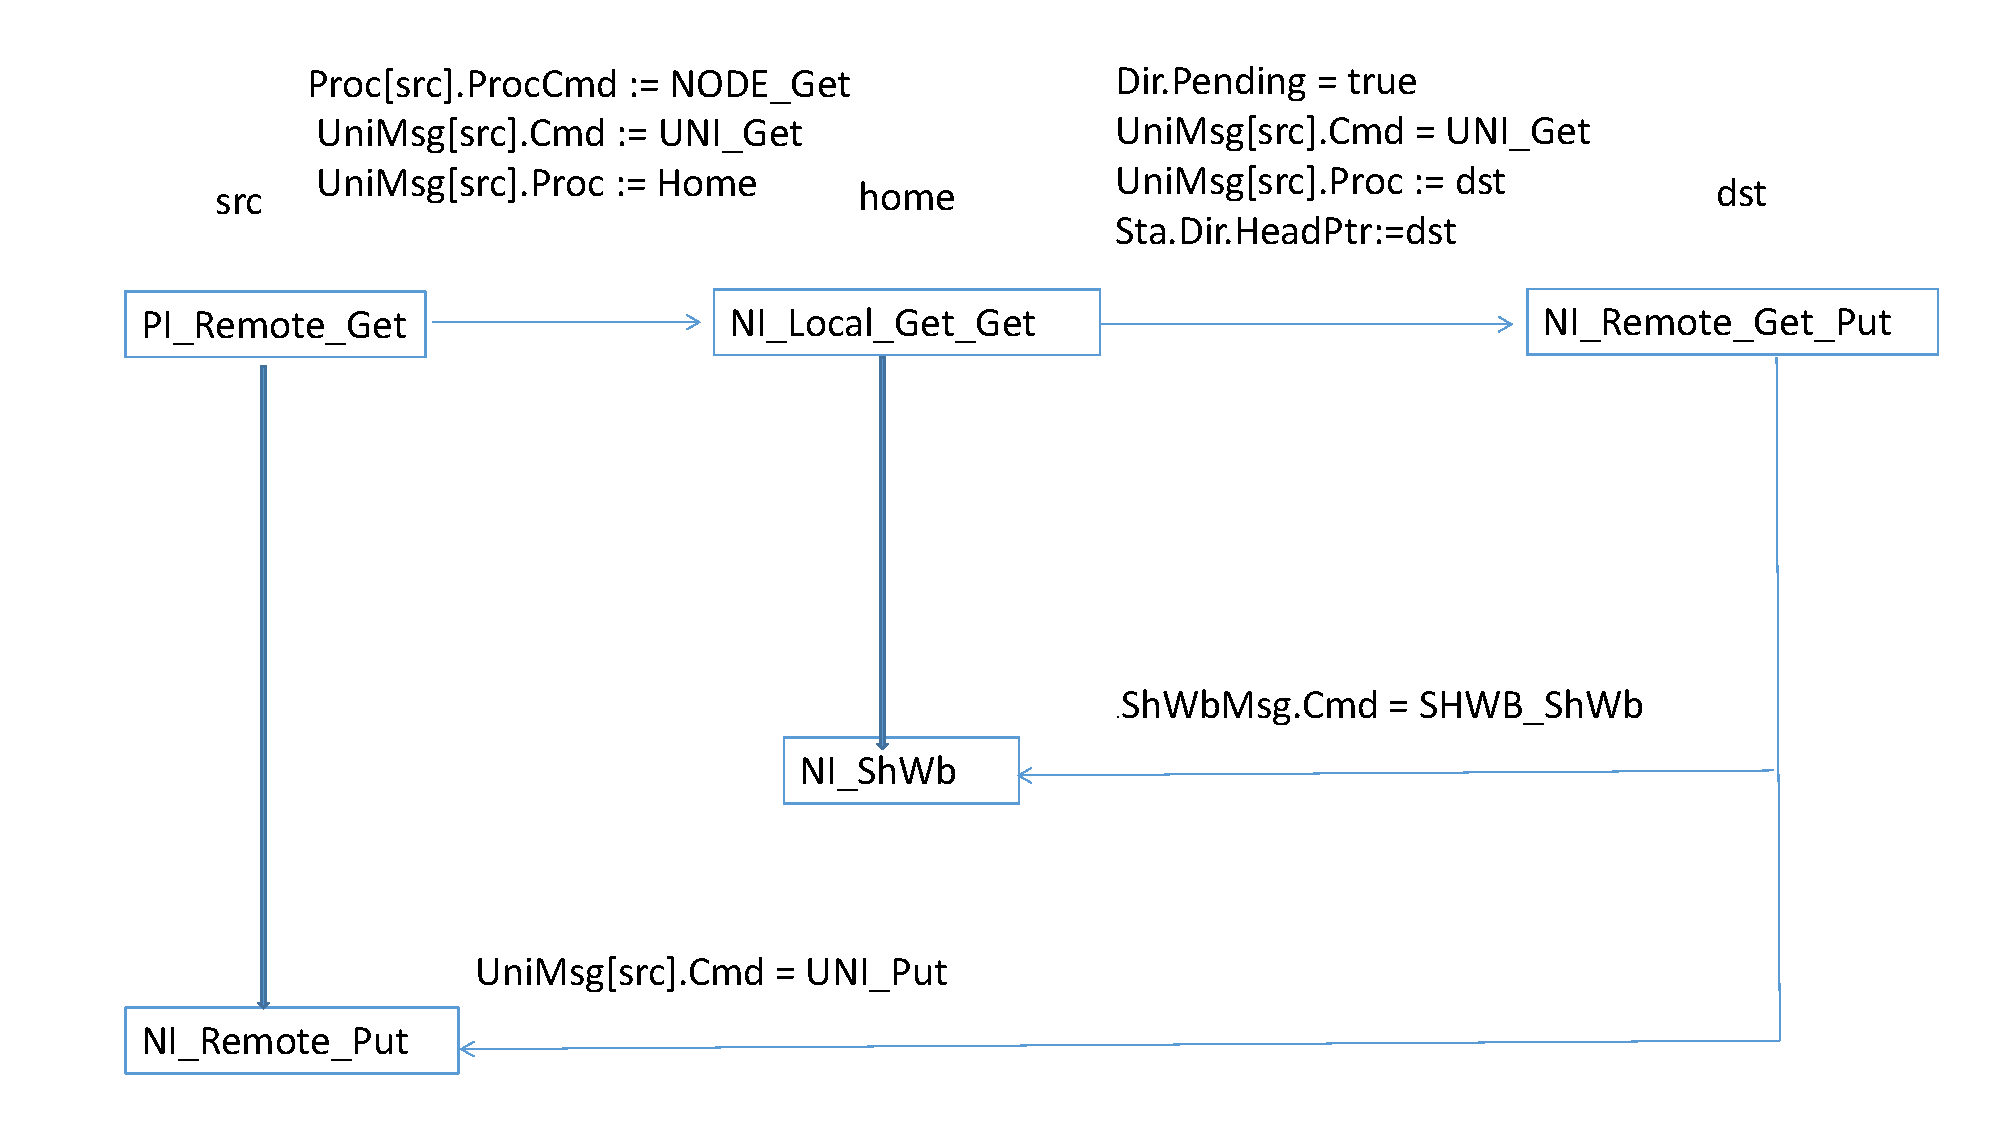
\includegraphics[width=1\textwidth]{flow2.pdf}

\caption{The flow of READ-transaction involving sharing-write back\label{fig:arch}
}
\end{figure}


This flow is finished by the following steps:
\begin{enumerate}
\item An idle remote  client $src$ needs a shared copy of a memory line, and executes   rule PI\_Remote\_Get,  sends the GET request to home.

\item  When the GET request from $src$ arrives at the
home, the home consults the directory to find that the line is dirty in $dst$,  executes rule NI\_Lcal\_Get\_Get: forwards the GET to $dst$ by telling that $src$ needs the data, and sets Dir.Pending TRUE to make no any other node's request to be processed during the sharing write-back procedure.

\item  When $dst$ receives the forwarded GET, the
processor $dst$ executes rule NI\_Remote\_Get\_Put, sets its copy to shared state and issues a PUT to $src$ conveying the dirty data,  and  issues a   shwb\_shwb
 (sharing write-back) conveying the dirty data at the same time.

\item   When $home$ receives this SHWB message, it executes the rule NI\_ShWb,
 writes the received
data back to main memory and puts $src$ on the sharer list.

\item When $dst$ receives this PUT message, it executes the rule NI\_Remote\_Put. If there is not another INV message, then it   uses the received data to update its cache line, and sets its cache to shared state.


\end{enumerate}

In order to understand state transitions of this flow after shwb\_shwb is issued, we may observe the invariants containing the condition Sta.ShWbMsg.Cmd = shwb\_shwb.

\begin{specification}\\
inv\_\_13: !((!(Sta.ShWbMsg.Data = Sta.CurrData)) \& (Sta.ShWbMsg.Cmd = shwb\_shwb))\\
inv\_\_21: !((Sta.Proc[1].CacheState = cache\_e) \& (Sta.ShWbMsg.Cmd = shwb\_shwb))\\
inv\_\_26: !((Sta.ShWbMsg.Cmd = shwb\_shwb) \& (Sta.HomeProc.CacheState = cache\_e))\\
inv\_\_29: !((Sta.ShWbMsg.HomeProc = TRUE) \& (Sta.ShWbMsg.Cmd = shwb\_shwb))\\
inv\_\_34: !((Sta.UniMsg[1].Cmd = uni\_putx) \& (Sta.ShWbMsg.Cmd = shwb\_shwb))\\
inv\_\_42: !((Sta.ShWbMsg.Cmd = shwb\_shwb) \& (Sta.Dir.Dirty = FALSE))\\
inv\_\_43: !((Sta.ShWbMsg.Cmd = shwb\_shwb) \& (Sta.HomeUniMsg.Cmd = uni\_putx))\\
inv\_\_49: !((Sta.ShWbMsg.Cmd = shwb\_shwb) \& (Sta.Dir.Local = TRUE))\\
inv\_\_55: !((Sta.HomeUniMsg.Cmd = uni\_put) \& (Sta.ShWbMsg.Cmd = shwb\_shwb))\\
inv\_\_56: !((Sta.WbMsg.Cmd = wb\_wb) \& (Sta.ShWbMsg.Cmd = shwb\_shwb))\\
inv\_\_57: !((Sta.ShWbMsg.Cmd = shwb\_shwb) \& (Sta.Dir.Pending = FALSE))\\
inv\_\_58: !((Sta.ShWbMsg.Cmd = shwb\_shwb) \& (Sta.HomeUniMsg.Cmd = uni\_getx))\\
inv\_\_70: !((Sta.HomeUniMsg.Cmd = uni\_get) \& (Sta.ShWbMsg.Cmd = shwb\_shwb))\\
inv\_\_75: !((Sta.ShWbMsg.Cmd = shwb\_shwb) \& (Sta.Dir.InvSet[1] = TRUE))\\
inv\_\_76: !((Sta.ShWbMsg.Cmd = shwb\_shwb) \& (Sta.NakcMsg.Cmd = nakc\_nakc))\\
inv\_\_101: !((Sta.UniMsg[1].Cmd = uni\_get) \& (Sta.UniMsg[1].HomeProc = FALSE) \&\\ ~~~~(Sta.ShWbMsg.Cmd = shwb\_shwb))\\
inv\_\_102: !((Sta.ShWbMsg.Cmd = shwb\_shwb) \& (Sta.Dir.ShrSet[1] = TRUE))\\
inv\_\_104: !((Sta.ShWbMsg.Cmd = shwb\_shwb) \& (Sta.Dir.ShrVld = TRUE))\\
inv\_\_105: !((Sta.ShWbMsg.Cmd = shwb\_shwb) \& (Sta.UniMsg[1].Cmd = uni\_getx) \&\\~~~~(Sta.UniMsg[1].HomeProc = FALSE))\\
inv\_\_135: !((Sta.Dir.HeadVld = FALSE) \& (Sta.ShWbMsg.Cmd = shwb\_shwb))\\
inv\_\_146: !((Sta.Dir.HomeHeadPtr = TRUE) \& (Sta.ShWbMsg.Cmd = shwb\_shwb))\\
\end{specification}

inv\_\_13 says that Sta.ShWbMsg.Data must be the same as Sta.CurrData because $dst$ conveys the dirty data when it issues the  shwb\_shwb command in executing rule NI\_Remote\_Get\_Put. At the same time, $dst$ also sets its copy to shared state, thus there is no an exclusive copy. This specified by inv\_\_21 and inv\_\_26. Because   $src$ is a remote node, Sta.ShWbMsg.HomeProc is set FALSE. This is formalized by inv\_\_29. Because  a sharing write-back occurs in a READ-transaction, and others' requests are pended to be processed, there will be no any uni\_putx command  to grant a node's WRITE-request. This formalized by inv\_\_34 and inv\_\_43. Home node itself will not grant its local WRITE-request, thus Sta.HomeUniMsg.Cmd  can't be  uni\_getx. Due to the pending status, thus replacement to the exclusive copy and invalidating operation to shared nodes can't occur, thus Sta.WbMsg.Cmd can't be wb\_wb, Sta.NakcMsg.Cmd can't be nakc\_nakc, and Sta.Dir.InvSet tag to any node can't be TRUE. These are formalized by inv\_\_56, inv\_\_76, and inv\_\_102.  A sharing write-back occurs when Home node find that there is a remote and dirty copy, therefore Sta.Dir.Dirty must be TRUE and Sta.Dir.Local must be FALSE. This is formalized by inv\_\_42 and inv\_\_49. A dirty copy also means that no any other node shares this data, thus Sta.Dir.ShrSet of any node is set FALSE. This is formalized by inv\_\_75.  At the same time, Sta.Dir.HeadVld has been set TRUE and Sta.Dir.HomeHeadPtr has been set to $dst$. This formalized by inv\_\_135 and inv\_\_146 respectively. At the same time,


\section{Conclusion\label{sec:conclusion}}
%=========================================
Our case studies on cache coherence protocols are typical examples
to illustrate the guiding principle of {\sf paraVerifier}. The
 consistency lemma based on the induction approach, is the
core of our work, which gives the heuristics to guide the tool
 to search invariants. Instead of ``invisible invariants" in previous work
 (see e.g,~\cite{Pnueli2001}, our invariants are visible,
 which can be further refined to precisely
 analyze the correctness of the protocol both in theoretical and practical aspects.

\bibliographystyle{splncsnat}
\bibliography{gste,cache,refer}
\end{document}
